\chapter{The Auger Process}\label{ch:auger}
The Auger process was first explained by  Pierre Auger in 1923 who was performing experiments with X-rays in a cloud chamber. He observed that besides the photoelectrons, which had an energy dependent on the energy of the X-rays, there were also emitted electrons with a constant energy and thus independent on which source had been used. These so-called radiationless transitions were due  to the relaxation of the electron holes in the atom created by the photoemission process. We shall from here on refer to these processes as Auger transitions. The process is illustrated in \autoref{fig:aes}.

The {\em initial state} in this case consists of an atom where a hole has been created in a deep-lying core level. As we shall see, it is not interesting how this initial state was created. This atom is now highly excited and will eventually undergo a relaxation process. In Chapter \ref{ch:xps} we saw that this relaxation can lead to emission of an X-ray photon, however, as long as the binding energy of the initial hole is well below \SI{10}{k\electronvolt} this process has a rather low probability of taking place. It is actually much more likely that a  weakly bound electron will drop down and fill the initial hole and instead of emitting a photon use the energy to excite another electron out of the atom, leading to the {\em final state}. As  shown in \autoref{fig:aes} the final state consists of an atom with two holes either in some core levels, or in the  valence  levels or any combination thereof.

As for the photoemission process, the  kinetic energy of the emitted electron will simply be the difference between the initial state and the final state. A crude estimate will thus be given by the Koopman binding energies as

\begin{equation}\label{eq:ekinkoopman}
E_{kin}=E_{initial}-E_{final}\approx E_{B          initial}-E_{Bfinal1}-E_{Bfinal2}
\end{equation}

\noindent where $E_x$ refers to the one electron binding energy of the holes involved.

Just as in the case of XPS it is clear that the energy distribution of the emitted electron will provide a unique identification of which elements and how much of each is present in our sample. If the appropriate energy interval is chosen it will also be surface sensitive. Thus we have a method which is very  similar  to XPS. However, there are a number of differences which sometimes makes AES more useful than XPS or vice versa.

\begin{figure}[h!]
	\begin{center}
	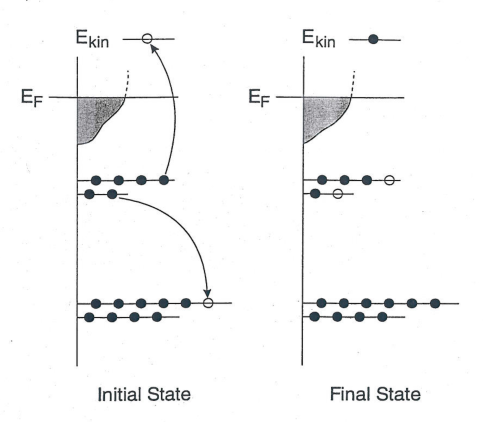
\includegraphics[scale=2.5]{figures/06_01.png}
	\caption{Sketch of an  Auger  process. Notice that both initial and final states have two holes.}
	\label{fig:aes}
	\end{center}
\end{figure}

\section{The Excitation Source}\label{sec:aessource}
The major difference between AES and XPS is the manner in which we get the atoms to emit electrons. We have earlier seen (see Fig. \ref{fig:cuxps}) that there will always be emitted Auger electrons as a result of the relaxation of the holes created by the photoemission process. This is however a very inconvenient way of generating the necessary initial holes for the Auger process. It is much more useful to use a high energetic electron beam typically from \SIrange{3}{10}{k\electronvolt}. As we saw under the discussion of the various energy loss mechanisms, energetic electrons will have a finite possibility of ionising the atoms in the substrate and hereby creating the necessary initial holes in a deep-lying core level (see Fig. \ref{fig:discrete_losses}). The advantage of using an electron beam is that it can be focused and manipulated rather well and still have a high current density.
        
The electron beam is generated by use of an electron gun which is usually mounted inside the CMA as indicated in \autoref{fig:schematics_cma}. By passing current through a filament it will be heated sufficiently so that electrons can evaporate and be accelerated towards the sample. A number  of lenses ensure that the beam diameter can be controlled and deflection plates at the end of the gun ensures that the beam can be manipulated to any desired position on the surface or scan over an area (see Fig. \ref{fig:aesschem}).

\begin{figure}[h!]
	\begin{center}
	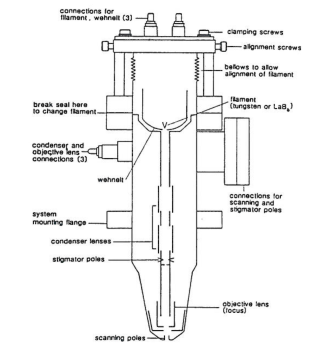
\includegraphics[scale=4]{figures/06_02.png}
	\caption{Schematics of an electron gun for AES.}
	\label{fig:aesschem}
	\end{center}
\end{figure}

As the lens system in the electron gun is an electrostatic imaging of the electron source onto the sample it is advantageous to use a \ce{LaB6} source. By mounting a \ce{LaB6} crystal on a filament a very good point source can be obtained and a spot diameter down to \SI{200}{\angstrom} can be achieved with a current of \SI{0.1}{nA}. Actually even higher resolutions can be obtained as in the  electron microscopes, but here we must remember that a sufficiently high current density is required if we want to obtain Auger spectra with a reasonable signal to noise ratio. As this demands no less than \SI{0.1}{nA} and as it is not possible to  confine electrons to spots smaller than \SI{200}{\angstrom} at such high  current  densities (unless going to much higher energies which then causes other problems) this in reality sets the limit for lateral resolution in AES.

\section{The Fine Structure in AES}
As mentioned the kinetic energy of the Auger electrons is given by the difference between the initial and final state. Thus Eq. \eqref{eq:ekinkoopman} is only very crude as we know that the atom will undergo relaxations when the initial  hole is being created. A better approximation is therefore to take the binding energy of the two final holes to be an average of the binding energy for the atom considered $Z$ and the binding energy it would have in an atom with $Z+1$. The kinetic energy could then be approximated by

\begin{equation}
E_{kin}\approx E_{Binitial}^Z-\frac{E_{Bfinal1}^{Z+1}+E_{Bfinal1}^Z+E_{Bfinal2}^{Z+1}+E_{Bfinal2}^Z}{2}
\end{equation}

\noindent where $E_x^Z$ refers to the one electron binding energy of the hole $x$ in atom $Z$. In \autoref{fig:aestrans} the kinetic energy for the strongest Auger lines is given for most of the elements. It is obvious that it is nearly always possible to find an Auger line with an energy in the interval where the electrons will be surface sensitive.

\subsection{Nomenclature}
An Auger transition is always named XYZ describing which energy levels are participating in the transition. The X refers to the initial hole, whereas the Y and Z refers to the two holes in the final state. In order to make this more complicated than necessary the old X-ray  notation is used for these levels. Here the various levels have the following names:

\vspace{0.5cm}

             \noindent   1s   \hfill   K\\   2s,   2p$_{\frac{1}{2}}$,
          2p$_{\frac{3}{2}}$ \hfill L$_1$,  L$_2$,  L$_3$\\  3s,
          3p$_{\frac{1}{2}}$, 3p$_{\frac{3}{2}}$,  3d$_{\frac{3}{2}}$,
          3d$_{\frac{5}{2}}$   \hfill   M$_1$,   M$_2$,   M$_3$,
          M$_4$,       M$_5$\\       4s,       4p$_{\frac{1}{2}}$,
          4p$_{\frac{3}{2}}$, 4d$_{\frac{3}{2}}$,  4d$_{\frac{5}{2}}$,
          4f$_{\frac{5}{2}}$,   4f$_{\frac{7}{2}}$   \hfill   N$_1$,
          N$_2$,  N$_3$,  N$_4$,  N$_5$,  N$_6$,   N$_7$\\
          
\begin{figure}[h!]
	\begin{center}
	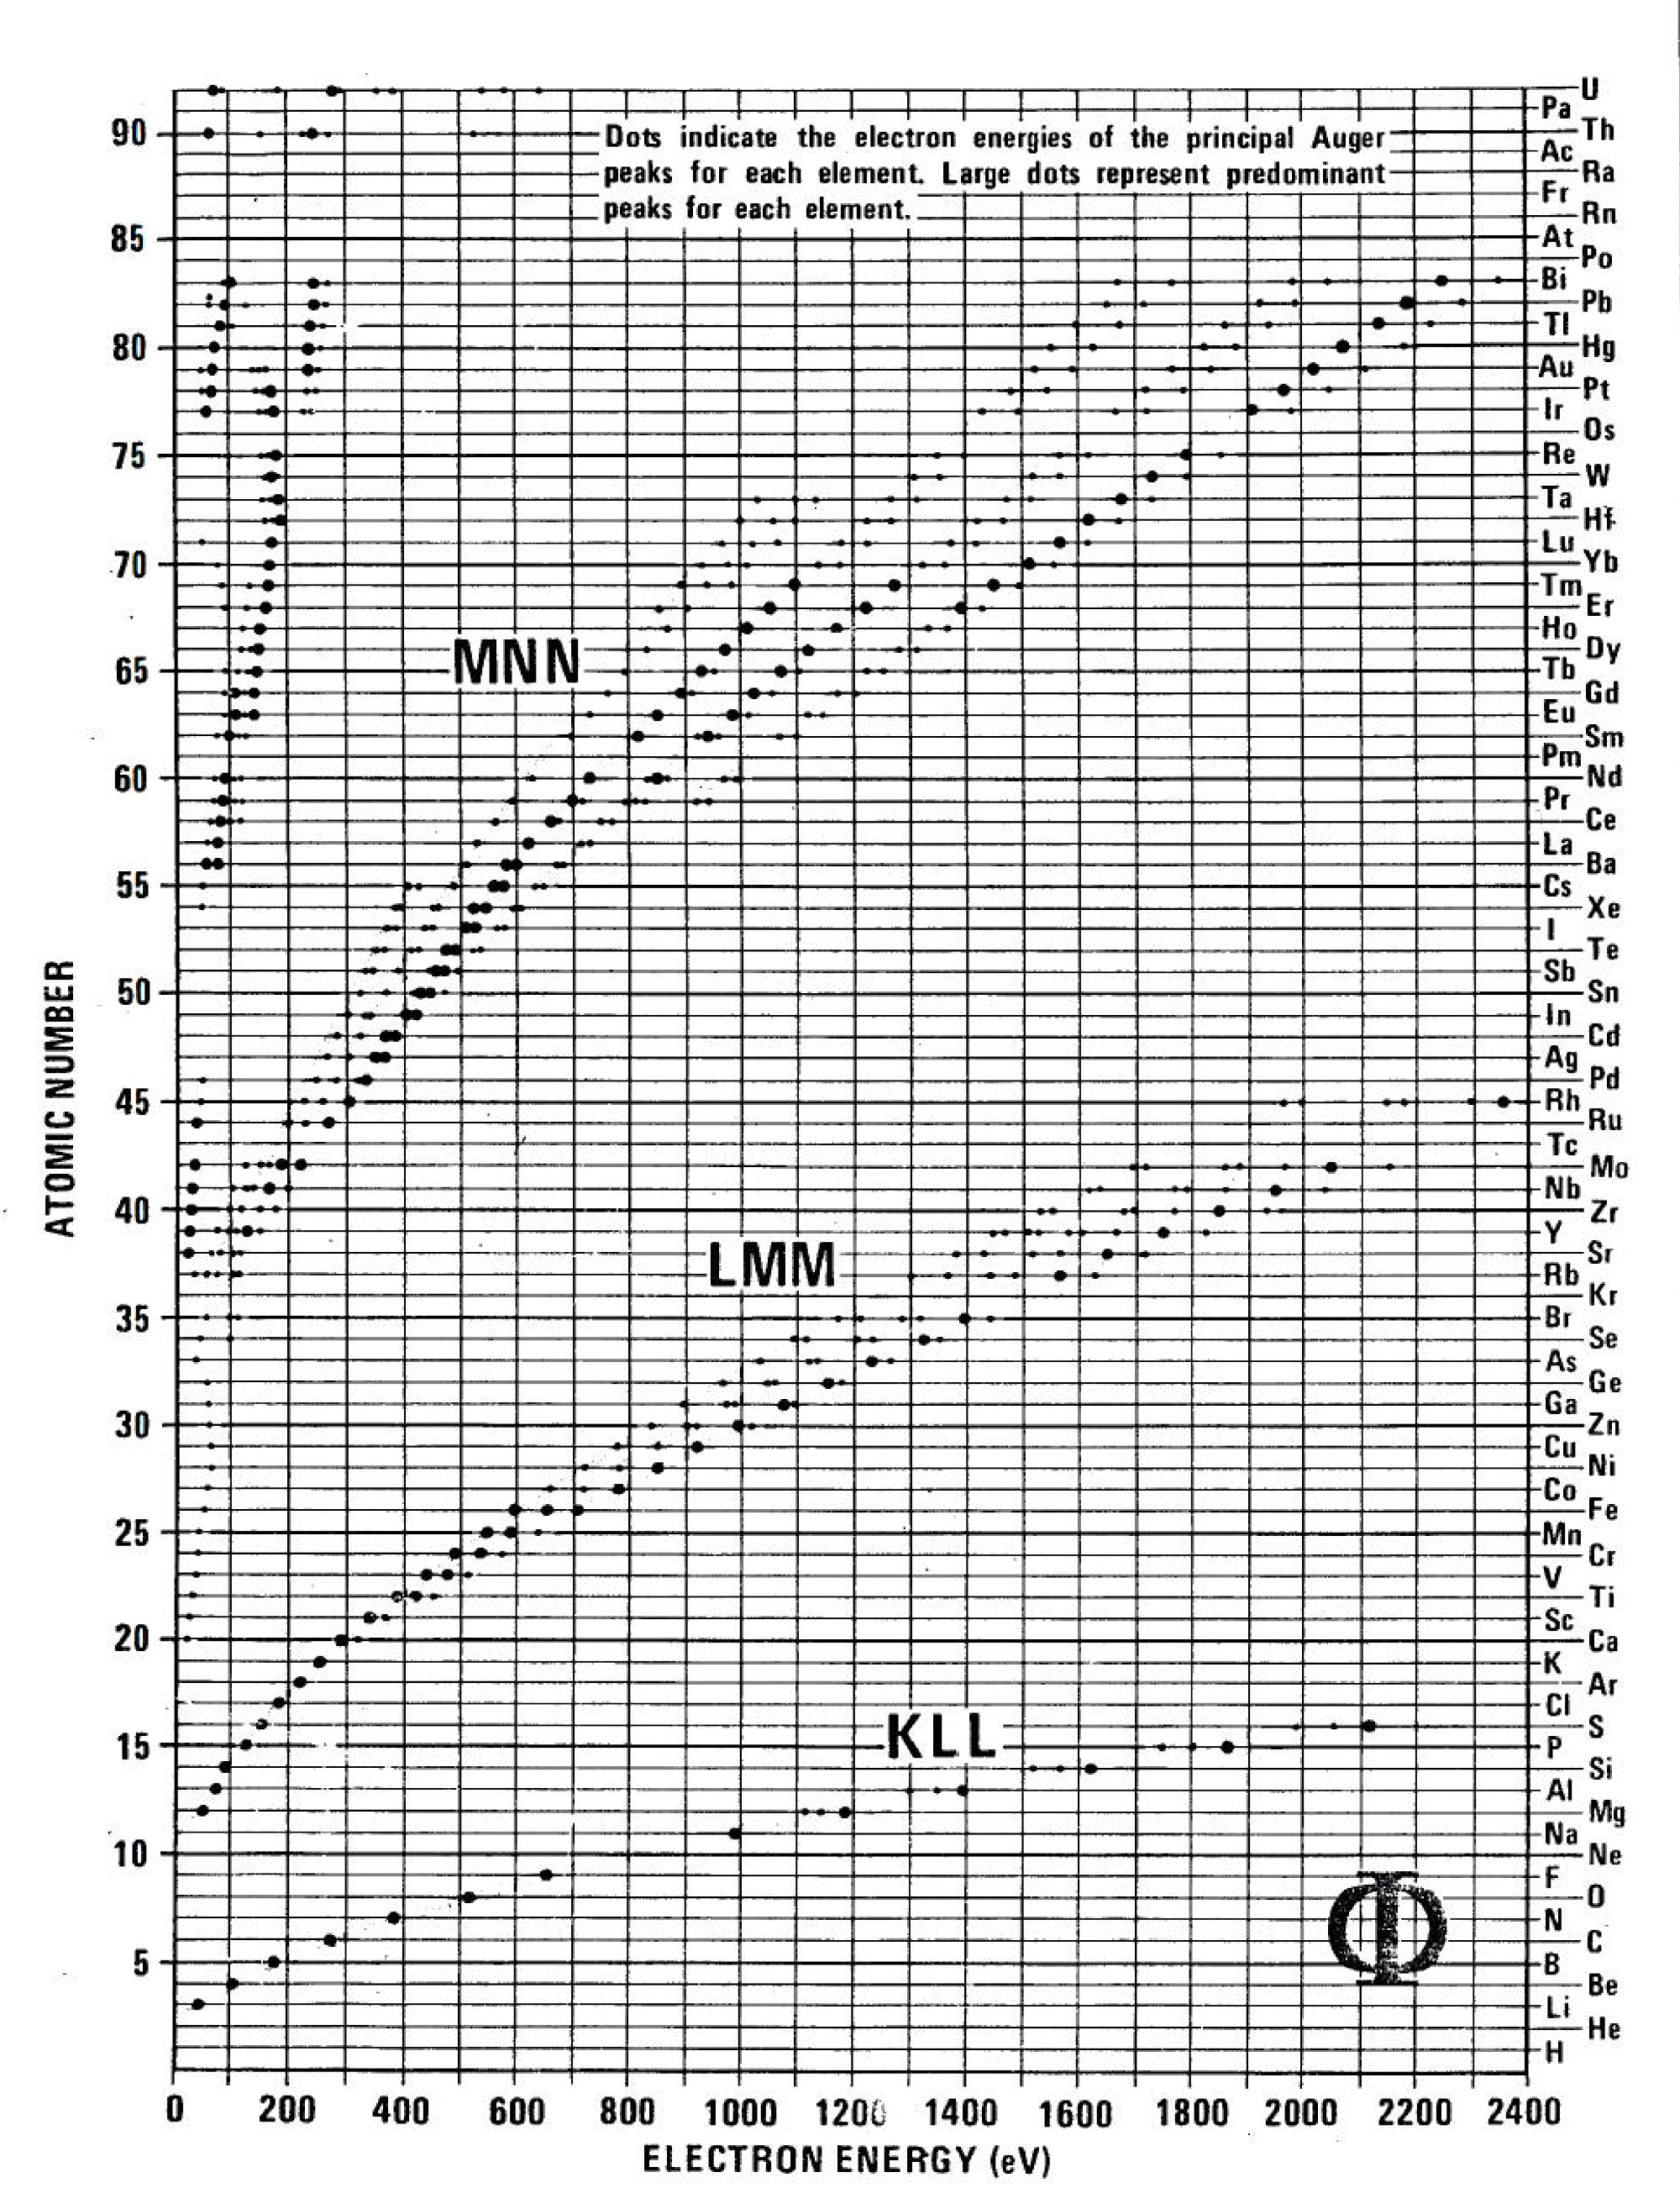
\includegraphics[width=0.95\textwidth]{figures/stronges_auger_lines.png}
	\caption{Energies of the strongest Auger transitions.}
	\label{fig:aestrans}
	\end{center}
\end{figure}

\subsection{Mulitiplet Splitting in AES}
If we consider a transition starting with  a hole in the 1s shell which results in two holes in the 2s or 2p shell then the name of the transition would be KLL which is the dominant type of lines for the lighter elements. This type of transition can naturally be divided up into different combinations like: KL$_1$L$_1$, KL$_1$L$_2$, KL$_1$L$_3$, KL$_2$L$_3$, KL$_2$L$_2$, KL$_3$L$_3$ leading to six lines.

In \autoref{fig:mgaes} this type of transition is shown for magnesium and it is easily seen that the spectrum cannot be explained by only four lines. The reason that we only got six lines is that we used a notation  only appropriate in jj-coupling. We saw earlier that when more than one localised hole is present it is more appropriate to use intermediate coupling starting either from jj-coupling or LS-coupling.

\begin{figure}[h!]
	\begin{center}
	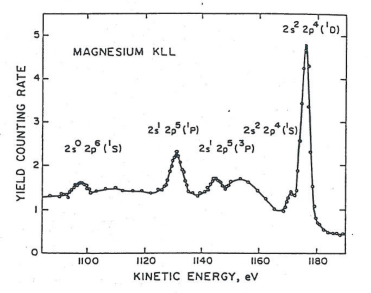
\includegraphics[scale=4]{figures/06_04.png}
	\caption{A KLL Auger spectrum of magnesium.}
	\label{fig:mgaes}
	\end{center}
\end{figure}

Thus in the intermediate coupling scheme the above transitions would lead to the following final states:

             \vspace{0.5cm}

          \noindent     KL$_1$L$_1$      \hfill      $^1S_0$\\
          KL$_1$L$_2$,           KL$_1$L$_3$            \hfill
          $^1P_1$,$^3P_0$,$^3P_1$,$^3P_2$\\
          KL$_2$L$_3$, KL$_2$L$_2$,  KL$_3$L$_3$   \hfill
          $^1S_0$,$^3P_0$,$^3P_1$,$^3P_2$,$^1D_2$\\

          \vspace{0.5cm}

Thus the simplest transition we can think of consists of a substantial number of lines. If the initial state is not an s-electron there will also be a splitting of the initial state due to a spin orbit splitting doubling the number of Auger lines. An example of this type of transition is shown in \autoref{fig:ybauaes} where the M$_{45}$N$_{67}$N$_{67}$ for ytterbium and gold are shown. The spin-orbit splitting of the N$_{45}$ level is very large in both cases leading to two well-separated multiples. A theoretical description of the line shape (using the intermediate coupling  scheme) is possible for the gold, but not for the ytterbium where other types of Auger transitions obscure the comparison. Due to an M$_{4}$M$_{5}$N$_{67}$ there will be a transition starting with a hole both in the M$_{5}$ and the N$_{67}$ level leading to a multiplet structure right on top of the M$_{5}$N$_{67}$N$_{67}$ lines. The spectra shown in \autoref{fig:ybauaes} was actually induced by the continuous bremsstrahlung emitted from an aluminium anode.

\begin{figure}[h!]
	\begin{center}
	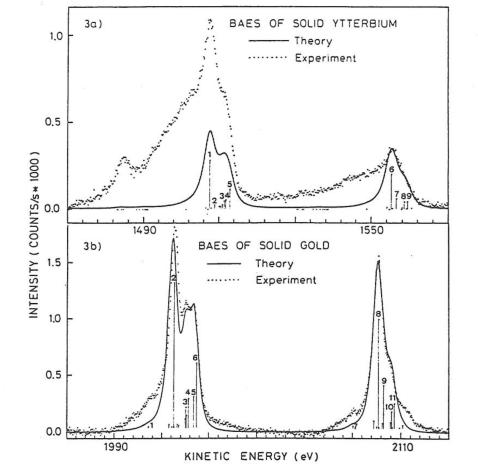
\includegraphics[scale=4]{figures/06_05.png}
	\caption{The experimental Auger spectra of Yb and Au and the theoretical fits.}
	\label{fig:ybauaes}
	\end{center}
\end{figure}

So far we have not discussed the transition probability for the Auger transition. As the relaxation process is due to the Coulomb interaction between the involved electrons, the interaction Hamiltonian will be described by a Coulomb interaction and the transition probability will be given again by Fermi's golden rule. In the frozen core approximation and one-electron picture this results in \cite{wentzel}:

\begin{equation}
P_{Auger}=\frac{4\pi^2}{h}\vert \left< \Phi_{Initial}\vert \frac{e^2}{r_{12}}\vert \Phi_{Final}\right>\vert ^2
\end{equation}

\noindent where initial and final states refers to the two vacancies in the initial and final state. This expression has been used to calculate the probability for going from each possible initial state to any available final state as shown in \autoref{fig:ybauaes}. In general the multiplet splitting of Auger transitions is quite complex leading to rather broad features as we have already seen. The lifetime broadening will contribute significantly as there are three holes involved in the process now. Furthermore, just as was  the case for the photoemission process, the Auger process will be followed by various shake-up and shake-off processes leading to satellite structures. They are therefore not as useful for chemical identification and investigations of electron structures as the XPS lines. But if we disregard the details of the structure and simply use the Auger lines as a finger print of the various elements they can be very useful.

\section{AES for Qualitative Analysis}
When creating a deep lying hole there are two competing possibilities for relaxation of the excited atom. One is the emission of a photon with the probability $\omega_{X}$, which was very useful for generation of X-rays for XPS, and the other is a decay through emission of an Auger electron with the probability $\omega_{Auger}$. The two channels are competing, but in general $\omega_{Auger}$ will be much larger than $\omega_{X}$ for initial holes with binding energy less than \SI{10}{k\electronvolt}. For example \autoref{fig:aesyield} shows the probability of the two types of  relaxation plotted for a hole in the 1s shell as a function of the atomic number. The binding energy of the 1s level in element $Z=33$ (As) is \SI{11.8}{k\electronvolt}. Thus for electron beams with energy less than \SI{10}{k\electronvolt} the Auger process will prevail.

\begin{figure}[h!]
	\begin{center}
	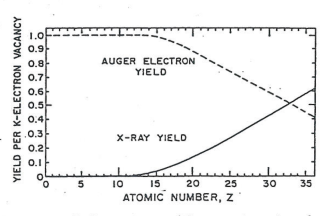
\includegraphics[scale=4]{figures/06_06.png}
	\caption{$\omega_{X}$ and $\omega_{A}$ as a function of Z for the 1s shell.}
	\label{fig:aesyield}
	\end{center}
\end{figure}

The emission of the X-rays actually has a  very useful aspect since they also carry information on which elements are present in the sample. This method is known by the name EDX and is mainly performed in combination with electron microscopy. It is complementary to the methods discussed here as it is not surface sensitive (usually probing $\sim \SI{1}{\micro m}$) on the atomic scale. Besides it is not a very useful method for detection of the light elements ($Z<11$) as most of the relaxation in this low binding energy regime takes place through Auger transitions.

An Auger spectrum of silver excited by the use of \SI{2}{k\electronvolt} electrons is shown in \autoref{fig:agaes}. The $N(E)$ spectrum is completely dominated by the elastically scattered electrons and primary electrons which have undergone energy losses in the solid.

\begin{figure}[h!]
	\begin{center}
	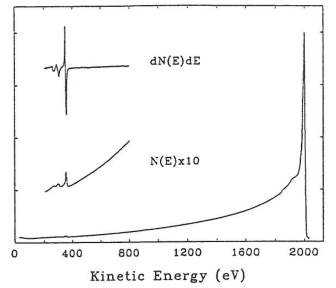
\includegraphics[scale=4]{figures/06_07.png}
	\caption{The raw N(E) spectra of silver excited by \SI{2}{k\electronvolt} electrons.}
	\label{fig:agaes}
	\end{center}
\end{figure}

Weak structures can be observed just below the elastic peak (energy loss features of silver) and around \SI{350}{\electronvolt}. This region has also been shown as $N(E)\times 10$ and it is now easily seen that there is a structure here. By consulting \autoref{fig:aestrans} these lines can be identified as the silver M$_{45}$N$_{45}$N$_{45}$ transition. The lines are lying on top of the high continuous background of secondary electrons which basically carries no information and it is therefore convenient to differentiate the spectrum as shown in the top panel. The nearly constant background is then eliminated and the structure of the line is easily recognised. The intensity of the lines, assuming a Gaussian line shape, can then be approximated by the peak to peak height. Just as for XPS all the Auger spectra of the elements have been collected in a handbook \cite{handbook} and Figures \ref{fig:alaes} and \ref{fig:al2o3aes} show a few examples of such standard Auger spectra.

\begin{figure}[h!]
	\begin{center}
	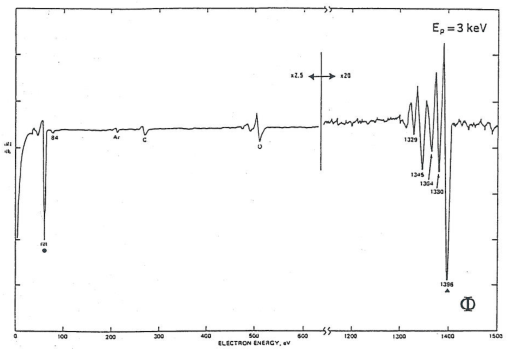
\includegraphics[scale=4]{figures/06_08.png}
	\caption{The standard Auger spectrum of aluminium.}
	\label{fig:alaes}
	\end{center}
\end{figure}

\autoref{fig:alaes} shows the Auger spectrum of a  relatively clean aluminium surface. Apart from several low level contamination features of Ar, C and O, two main features from aluminium are observed. The low lying line at \SI{68}{\electronvolt} is due to an L$_{23}$VV transition. The VV refers to the fact that the two final states are located in the valence band and the shape of the Auger line in this case will actually be a self-convolution of the valence band. The high energetic line at \SI{1396}{\electronvolt} is due to a KL$_{23}$L$_{23}$ transition which is much weaker. The features below \SI{1390}{\electronvolt} can be accounted for by energy losses due to plasmons. If this surface is oxidised to \ce{Al2O3} the spectrum undergoes rather strong changes as shown in \autoref{fig:al2o3aes}. Both transitions shift downwards in energy by \SIrange{17}{18}{\electronvolt} and the energy loss features change dramatically. This is a result of chemical shifts and changes in the relaxation mechanisms. The aluminium has by oxidation been changed from a very good conductor to an isolator. Thus the valence electrons have been shifted down in energy and there are no delocalised electrons around to effectively screen the excited final state. Therefore, the characteristic plasmon energy losses are no longer observed. In this case it is possible to identify the chemical state of the aluminium, especially when the presence of oxygen at \SI{510}{\electronvolt} is taken into account.

\begin{figure}[h!]
	\begin{center}
	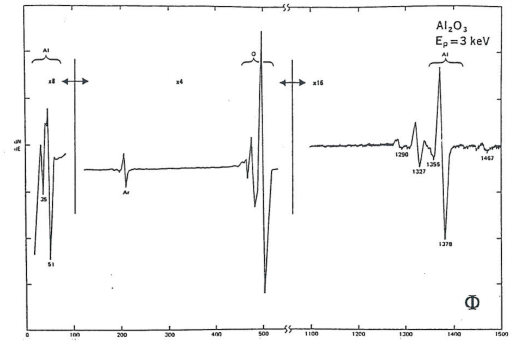
\includegraphics[scale=4]{figures/06_09.png}
	\caption{The standard Auger spectrum of \ce{Al2O3}.}
	\label{fig:al2o3aes}
	\end{center}
\end{figure}

Similar chemical identification can be done for carbon as seen in \autoref{fig:kllaes} where the carbon Auger feature is depicted for a number of carbon containing compounds. It is in general possible to differentiate between carbon in covalent bonding and ionic bonding. The carbides display a spectrum characteristic of a filled shell structure like neon. The same features are observed for nitrogen in nitrides and naturally for oxygen and fluorine. \autoref{fig:niaes} shows an AES study of the decomposition of methylamine on nickel. At very low temperatures the methylamine is chemisorbed associatively on the surface and the spectrum reflects the line shape expected from molecules to a high degree. As the surface is heated the molecule will decompose and finally all the hydrogen will desorb and the nitrogen and carbon will react with the surface forming carbides and nitrides which can easily be identified by their characteristic line shapes \cite{chorkendorff3}.

Thus chemical identification can sometimes be undertaken with AES, but certainly not as efficiently as with XPS. Besides there are other problems with AES  which should be mentioned when discussing chemical identification. Since a high energetic electron beam is used with a relatively high current density, there is always a potential danger that the excitation source itself introduces chemistry. This is not a severe problem for metals and alloys, but it is serious for chemical compounds like polymers or the methylamine shown above.

\begin{figure}[h!]
	\begin{center}
	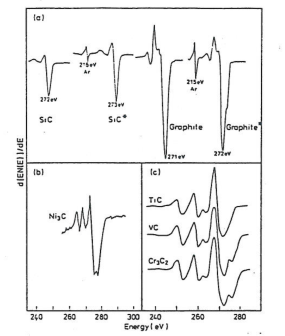
\includegraphics[scale=4.5]{figures/06_10.png}
	\caption{The Auger line shape of the KLL transition in various chemical surroundings.}
	\label{fig:kllaes}
	\end{center}
\end{figure}

\begin{figure}[h!]
	\begin{center}
	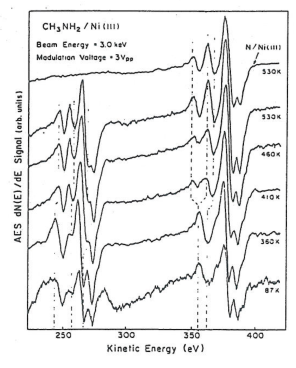
\includegraphics[scale=4]{figures/06_11.png}
	\caption{The Auger spectrum of methylamine adsorbed on Ni(111) during decomposition.}
	\label{fig:niaes}
	\end{center}
\end{figure}

If the AES spectrum of the chemisorbed  methylamine shown in the bottom of \autoref{fig:kllaes} was to be repeated after the surface had been exposed to the electron beam for 5 minutes the spectrum would look exactly as if it had reacted all the way to nickel-nitride and -carbide. Thus great care has to be taken when AES is used on compounds.

\section{AES for Quantitative Analysis}
Carrying out quantitative analysis with AES is very similar to XPS, although there are a few complicating factors. The probability for getting an Auger electron $XYZ$ out from a thin layer of element $x$ in the depth $z$ will be given by

\begin{equation}\label{eq:probxyz}
dI^{XYZ}_x(z)=N_x\sigma_X(z)\omega_{XYZ}e^{-\dfrac{z}{\lambda_{XYZ}}}i(z)T(E_{XYZ})dz
\end{equation}
          
\noindent where $N_x$ is the number of \si{atoms/cm^3}, $\sigma_X(z)$ is the cross section for generating the initial hole $X$ at depth $z$, $\omega_{XYZ}$ is the probability that the initial hole will decay as an Auger process, $\lambda_{XYZ}$ is the inelastic mean free path of the Auger electron, $T(E_{XYZ})$ is the probability that the electron will be detected by the analyser, $i(z)$ is the flux of primary electrons at depth $z$. The electron flux of primary electrons vary with the depth because these electrons will undergo energy losses and because they will scatter elastically in the solid. 

If we consider a pure element and assume that the dependency on depth is weak all these various factors can be put together in one constant namely
          
\begin{equation}
I^{\infty XYZ}_x=N_x\sigma_X\omega_{XYZ}i_0T(E_{XYZ})\lambda_{XYZ}
\end{equation}

\noindent which is the signal we will obtain from the clean sample. Equation \eqref{eq:probxyz} would then read

\begin{equation}
dI_x^{XYZ}(z)=\frac{I^{\infty XYZ}_x}{\lambda_{XYZ}}e^{-\dfrac{z}{\lambda_{XYZ}}}dz
\end{equation}

By integration from zero depth to infinity we get

\begin{equation}
I^{\infty XYZ}_x=\int dI_x^{XYZ}(z)=\int_0^{\infty}\frac{I^{\infty XYZ}_x}{\lambda_{XYZ}}e^{-\dfrac{z}{\lambda_{XYZ}}}dz 
\end{equation}

By measuring the signal from the pure elements it is possible to establish a set of sensitivity factors just as it was done for the XPS lines.

\begin{equation}
I^{XYZ}_x=S_x^{XYZ}N_x
\end{equation}
          
\noindent whereby the composition of a sample can be estimated as

\begin{equation}
C_x=\frac{I^{XYZ}_x}{S_x^{XYZ}\sum_i^N\frac{I^{XYZ}_i}{S_i^{XYZ}}}\times 100\%
\end{equation}
            
\noindent where the sum $i$ goes over all $N$ elements present in the sample.

The relative sensitivity factors for most of the strongest Auger lines are shown in \autoref{fig:aessf} for a primary electron beam of \SI{3}{k\electronvolt} and in \autoref{fig:aessf10kev} for a primary beam of \SI{10}{k\electronvolt}. Both figures are taken from \cite{handbook}.

\begin{figure}[h!]
	\begin{center}
	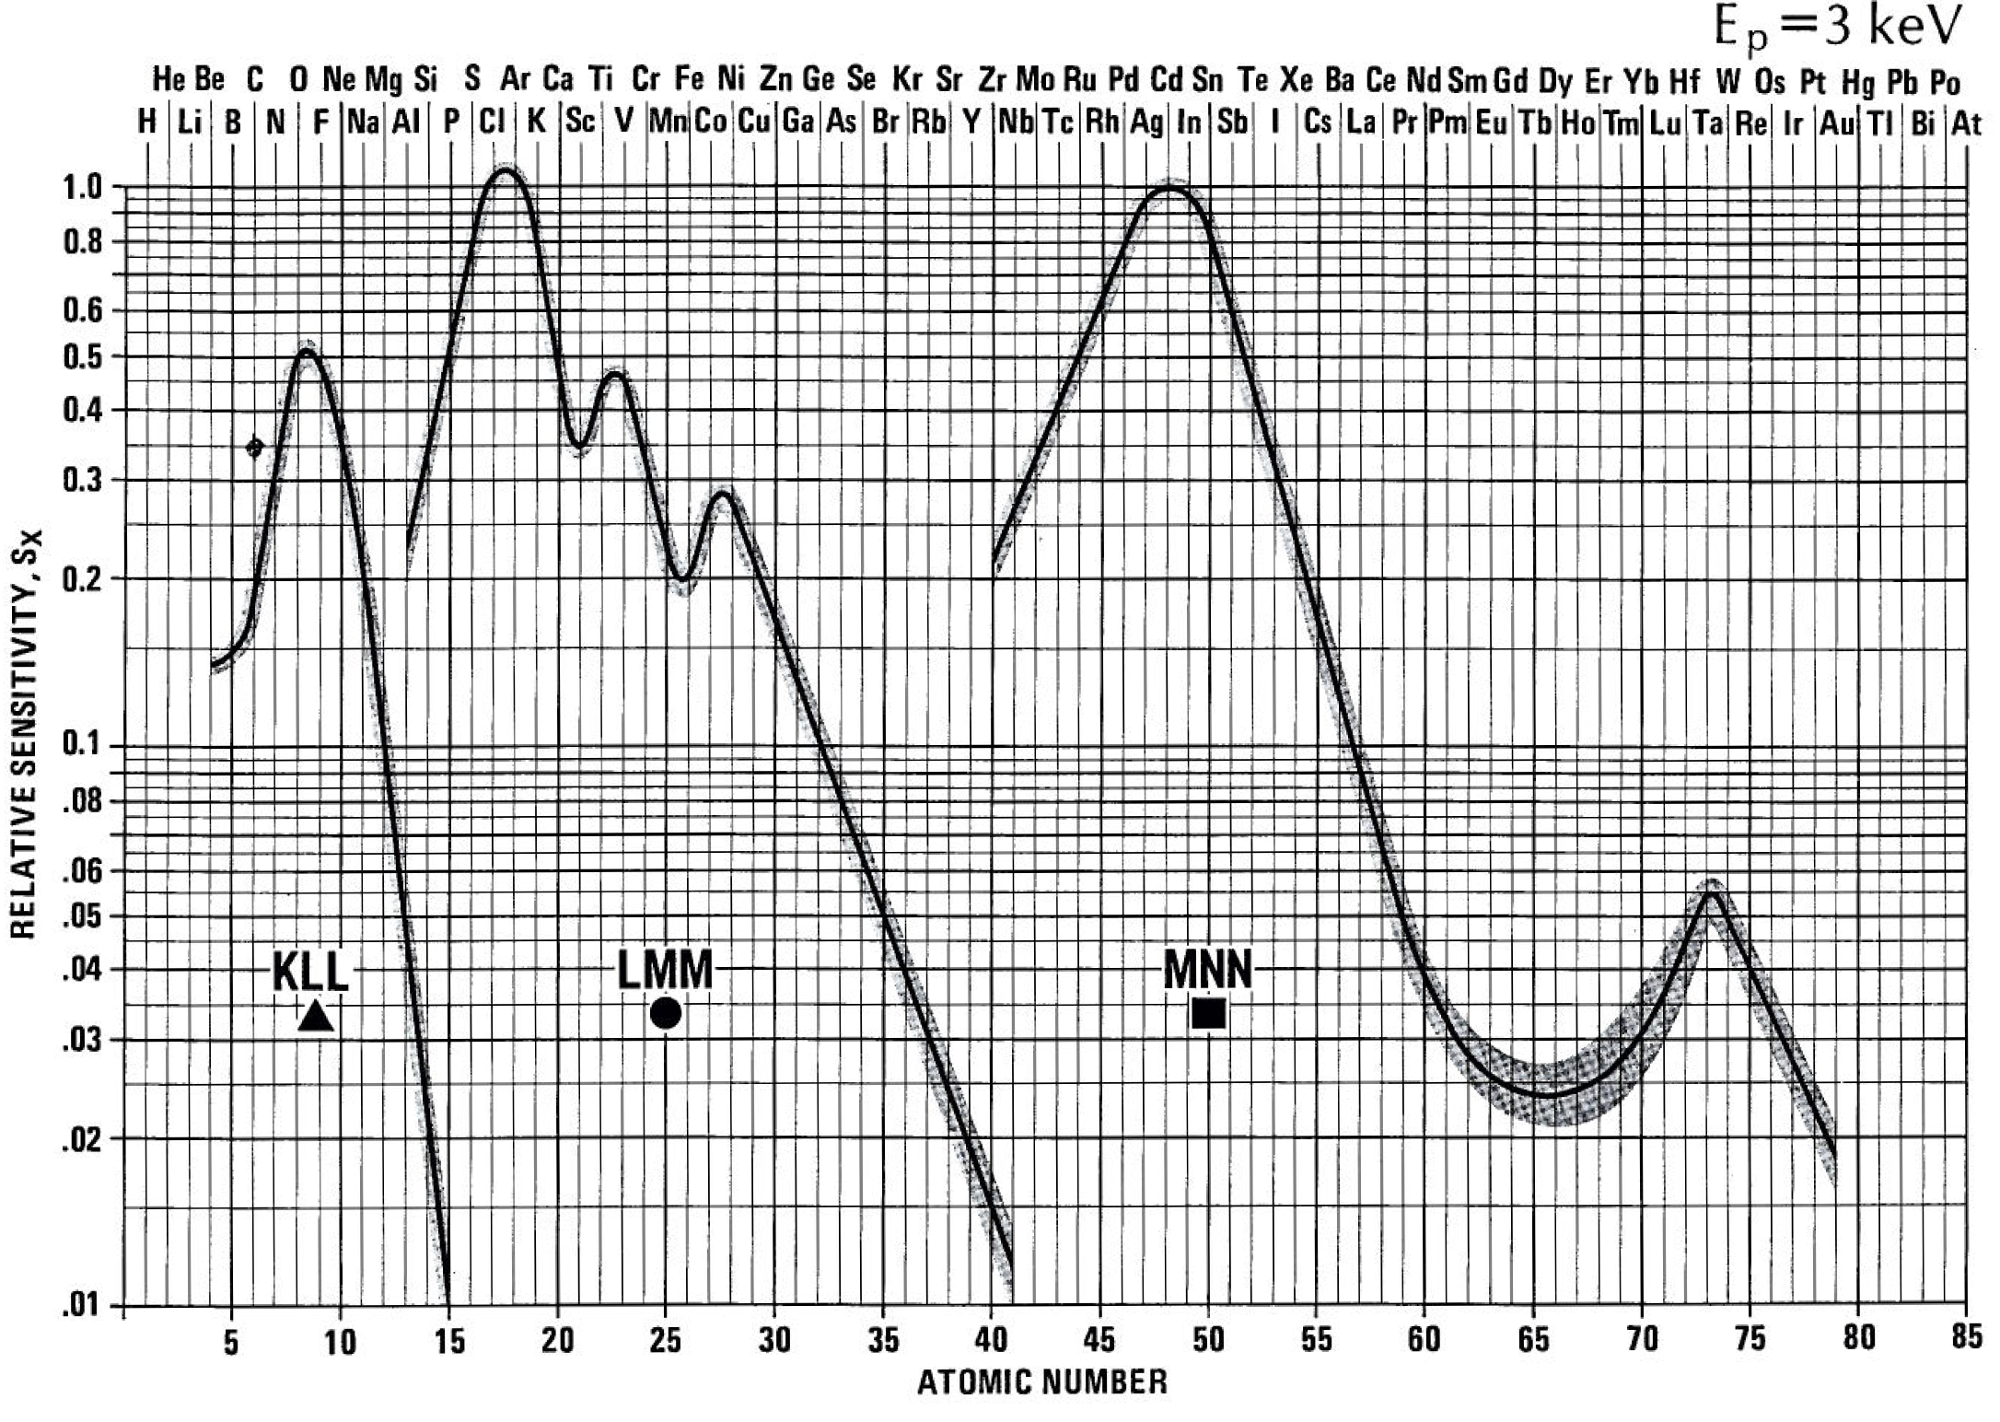
\includegraphics[width=0.95\textwidth]{figures/auger_sensitivity_3kev.png}
	\caption{The sensitivity factors for Auger transitions excited by \SI{3}{k\electronvolt} electrons.}
	\label{fig:aessf}
	\end{center}
\end{figure}

Several approximations were necessary to achieve this simple expression and the compositions determined in this manner will therefore also have a considerable uncertainty. Thus for investigations where accurate determination of the surface composition is mandatory XPS should be used. However, the AES method is very useful especially for determining relative compositions between different areas of the samples or depth analysis.

\begin{figure}[h!]
	\begin{center}
	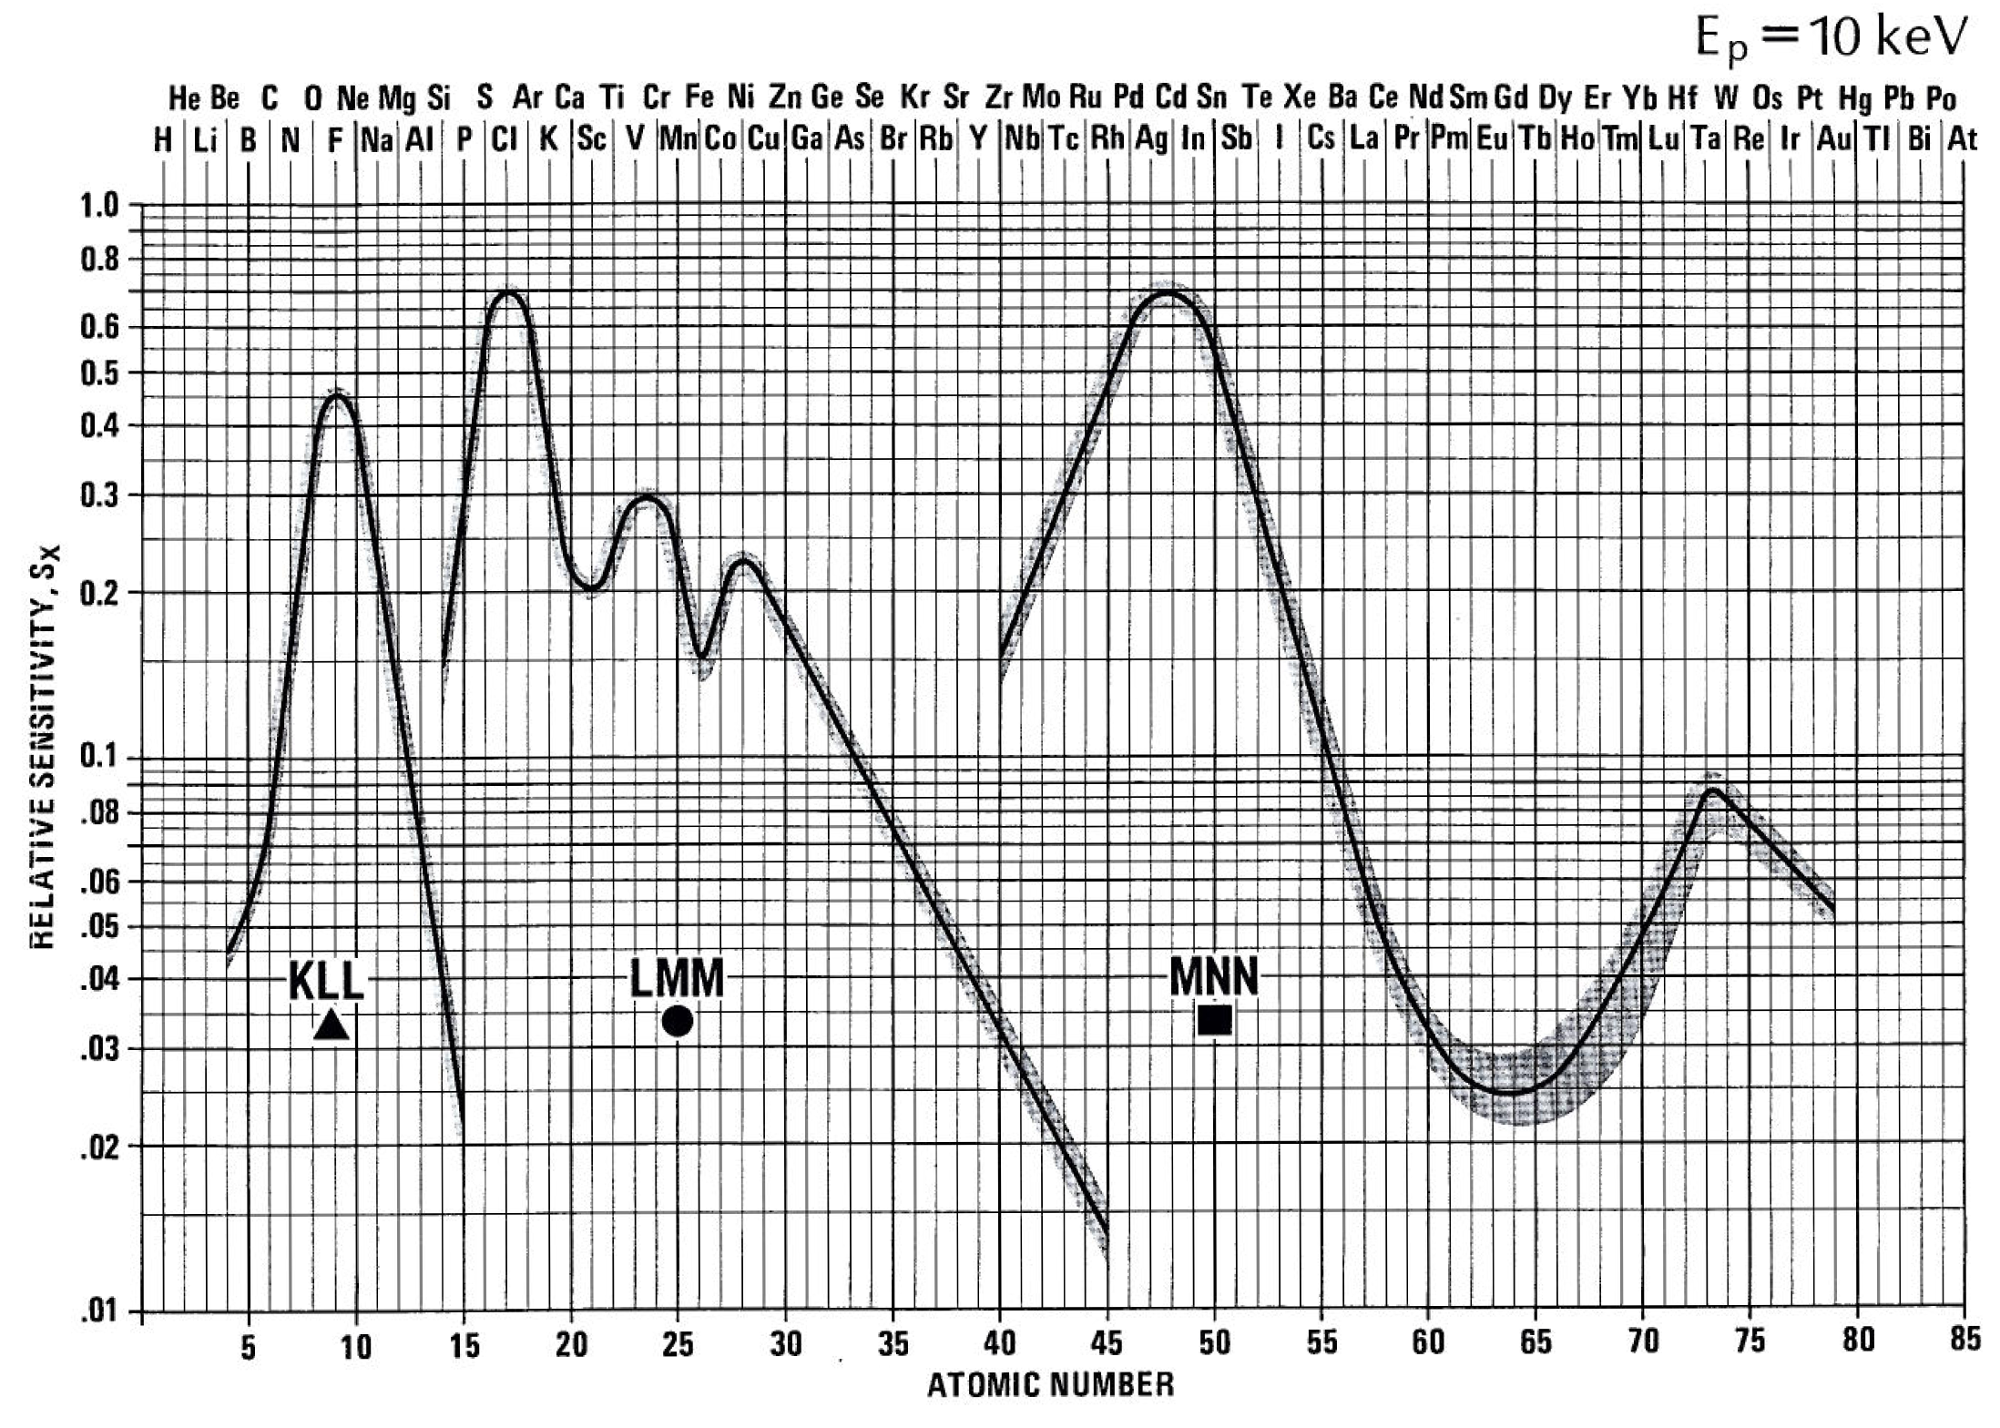
\includegraphics[width=0.95\textwidth]{figures/auger_sensitivity_10kev.png}
	\caption{The sensitivity factors for Auger transitions excited by \SI{10}{k\electronvolt} electrons.}
	\label{fig:aessf10kev}
	\end{center}
\end{figure} 

\subsection{Example}
In this example we shall demonstrate how the attenuation of the Auger signals can be used to study growth mechanisms on surfaces and how it can be used to determine the inelastic mean free path. \autoref{fig:gemvv} shows the natural logarithm of the Auger signal for two germanium lines relative to the pure germanium as a function of silicon coverage deposited on top of the germanium. It is seen that the germanium signal is damped exponentially. If we assume that the analyser was positioned normal to the surface we can estimate $\lambda$ for the two different kinetics energies if the coverage of the silicon is known and if we assume that it is deposited layer by layer. The germanium intensity will be given by

\begin{equation}\label{eq:gesignal}
I^{XYZ}_{\ce{Ge}}(d_{\ce{Si}})=I^{\infty XYZ}_{\ce{Ge}}e^{-\dfrac{d_{\ce{Si}}}{\lambda_{\ce{Si}}}}
\end{equation}

\noindent where $d_{\ce{Si}}$ is the thickness of the overlayer. The germanium signal will be damped through the silicon and it is therefore $\lambda_{\ce{Si}}$ which is determined in this manner.

\begin{figure}[h!]
	\begin{center}
	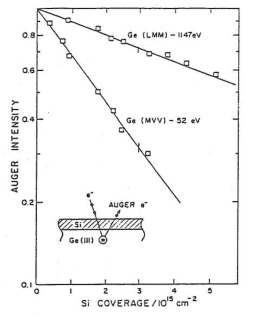
\includegraphics[scale=4.5]{figures/06_14.png}
	\caption{Attenuation of the Ge LMM (\SI{1147}{\electronvolt}) and Ge MVV (\SI{52}{\electronvolt}) Auger lines as a function of Si coverage.}
	\label{fig:gemvv}
	\end{center}
\end{figure}

By plotting $\ln(I^{XYZ}_{\ce{Ge}}(d_{\ce{Si}})/I^{\infty XYZ}_{\ce{Ge}})$ vs. $d_{\ce{Si}}$,  $\lambda_{\ce{Si}}$ can be found for the two energies.

Similarly the signal of the silicon Auger lines can be followed and the intensity of the silicon Auger lines would have the following form as a function of thickness

\begin{equation}\label{eq:sisignal}
I^{XYZ}_{\ce{Si}}(d_{\ce{Si}})=\int_0^{d_{\ce{Si}}}\frac{I^{\infty XYZ}_{\ce{Si}}}{\lambda_{\ce{Si}}}e^{-\dfrac{z}{\lambda_{\ce{Si}}}}dz=I^{\infty XYZ}_{\ce{Si}}(1-e^{-\dfrac{d_{\ce{Si}}}{\lambda_{\ce{Si}}}})
\end{equation}
          
The above results can easily be made more surface sensitive by changing the detection angle to be $\theta$ degrees off the normal. $\lambda$ would then in the above formulas change to $\lambda cos\theta$ as we saw in Equation \eqref{eq:intang}.

\subsection{Growth Mechanisms}
The ability to grow new structures on a substrate is a very important field in material science today. In the above example we assumed that the growth of the silicon was a layer by layer process. Thus one layer of Si is completed before the next layer is started and it is possible to grow perfect macroscopic crystal structures in this manner. If we look carefully at the germanium signal as a function of the silicon coverage, we shall see that the signal actually consists of a number of straight lines which form an exponential decay. The ratio of the germanium signal for a coverage of $\theta_{\ce{Si}}$ less than one monolayer will be given by

\begin{equation}
\frac{I_{\ce{Ge}}(\theta_{\ce{Si}})}{I_{\ce{Ge}}^{\infty}}=(1-\theta_{\ce{Si}})+\theta_{\ce{Si}}e^{-\dfrac{l_{\ce{Si}}}{\lambda_{\ce{Si}}}}\hspace{2cm}0\leq\theta_{\ce{Si}}\leq 1
\end{equation}

\noindent where $l_{\ce{Si}}$ is the thickness of one monolayer of silicon.

The above equation can easily be generalised to the transition from the $n^{th}$ layer to the $(n+1)^{th}$ layer

\begin{equation}
\frac{I_{\ce{Ge}}(\theta_{\ce{Si}})}{I_{\ce{Ge}}^{\infty}}=(1-\theta_{\ce{Si}})e^{-\dfrac{nl_{\ce{Si}}}{\lambda_{\ce{Si}}}}+\theta_{\ce{Si}}e^{-\dfrac{(n+1)l_{\ce{Si}}}{\lambda_{\ce{Si}}}}\hspace{2cm}0\leq\theta_{\ce{Si}}\leq 1
\end{equation}

\noindent where $\theta_{Si}$ is the amount of the $n^{th}$ layer covered with silicon.

The result of such an attenuation of the germanium signal is shown in \autoref{fig:geattenuation}.

\begin{figure}[h!]
	\begin{center}
	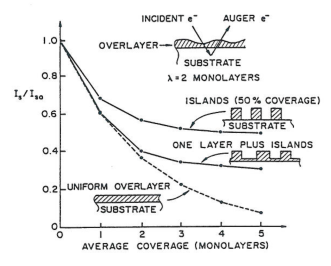
\includegraphics[scale=4]{figures/06_15.png}
	\caption{The attenuation of the substrate signal as a function of coverage. The different curves represents different growth mechanisms.}
	\label{fig:geattenuation}
	\end{center}
\end{figure}

Unfortunately the growth mechanisms are in general not as simple as we have just seen. They are dictated by surface diffusion, deposition rates, substrate temperature and surface and interface energies of the elements involved. It is beyond the scope of this review to go further into the various mechanisms, but we shall mention that there are other categories of growth.

\begin{itemize}
\item The layer by layer growth is called a {\bf Frank-van der Merwe growth}.
\item Another possibility is that the first layer is completed before the second layer is started, but then the layer by layer growth stops and islands are formed. This is called a {\bf Stranski-Krastanov growth} mode.
\item Finally there is the possibility that islands are formed right from the beginning and that is referred to as a {\bf Volmer-Weber growth} mode.
\end{itemize}

It is only in the first case it is possible to describe the process easily. In the other modes the unknown distribution of islands and their sizes makes an analysis very difficult. The effects of the various mechanisms are illustrated in \autoref{fig:geattenuation}.

Recent experiments using Scanning Tunnelling Microscopy, where it is possible to investigate the individual atoms deposited on the surface, have shown that alloying also complicates the above picture.

\section{Scanning Auger Microscopy SAM}
The biggest advantage of AES might be the ability to focus the primary electron beam on a small spot as we discussed in Section  \ref{sec:aessource}. Thus very small areas can be analysed. If this is combined with the possibility to scan the electron beam over the surface it is possible to obtain a lateral resolution of the surface composition.

\autoref{fig:cuagaes} shows an Auger spectrum of a copper grid placed on top of a silver foil. The distance between each mask of the grid is \SI{25}{\micro m} and the Auger spectrum was obtained while the electron beam was scanned over an area of $65\times\SI{100}{\micro m^2}$ with TV scan rate.

If the amount of secondary electrons emitted  from the surface is measured as a function of the beam position it is possible to construct an image of the surface. This is usually referred to as a secondary electron micrograph which can give topologic information of the surface. The top panel of \autoref{fig:cugrid} shows such a SEM picture of the copper grid.

If the analyser is now set to measure the intensity in a narrow window around, for example, the silver line at \SI{355}{\electronvolt} it is possible to measure the amount of silver in the surface as a function of the electron beam position. This is exactly what has been done in the rest of the panels in \autoref{fig:cugrid} for a number of the elements seen in \autoref{fig:cuagaes}. It is easily seen that the grid consists of copper and that it is placed on top of a silver foil. Furthermore it is observed that the contamination by sulphur is primarily located on the silver, whereas the chlorine is mainly adsorbed on the copper grid. The resolution in this picture is around \SI{1}{\micro m}.

\begin{figure}[h!]
	\begin{center}
	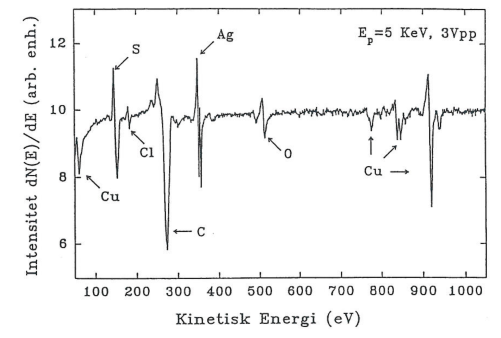
\includegraphics[scale=4]{figures/06_16.png}
	\caption{The Auger spectrum of a copper grid mounted on a silver foil and averaged over an area of 65$\times$100 \si{\micro m^2}.}
	\label{fig:cuagaes}
	\end{center}
\end{figure}

The methods can be refined by measuring not only the intensity of the Auger line, but also the intensity of the background before and after the peak. In this manner the (Signal-Background)/Background can be used for the imaging and hereby topologic effects will be reduced.

SAM is a rather time consuming process dependent on the resolution required and the size of the area investigated. In general at least \SI{10}{ms} is required for each point measured (dependent on the primary current and thus dependent on the resolution of the electron beam) and if a high resolution is needed $512\times512$ points may be required. Such a picture will then take \SI{2500}{seconds} and three times as long if the background needs to be eliminated.

The method is very useful in many contexts, especially in applied material science.

\begin{figure}[h!]
	\begin{center}
	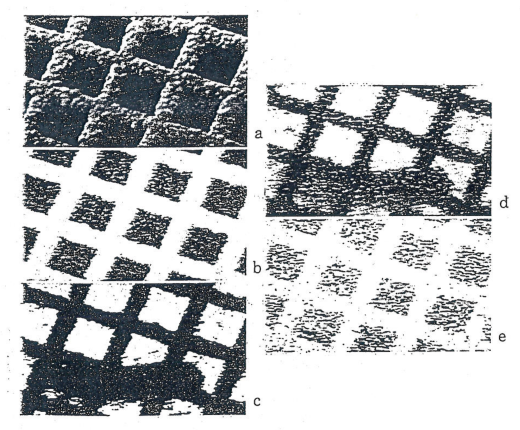
\includegraphics[scale=3]{figures/06_17.png}
	\caption{a)The SAM picture of a copper grid mounted on a silver foil. The first picture is a Secondary Electron Micrograph picture showing the  grid. Then follows the SAM pictures of b) Cu, c) Ag, d) S and e) Cl.}
	\label{fig:cugrid}
	\end{center}
\end{figure}

\section{Problems}
\begin{enumerate}
\item Estimate from \autoref{fig:gemvv} the mean free path for electrons with energies of \SI{52}{\electronvolt} and \SI{1147}{\electronvolt}, respectively, through Si.

How does this fit into the universal curve shown in \autoref{fig:mean_free_path}?

Discuss how the signals in \autoref{fig:gemvv} would behave if we did not have Frank-van der Merwe growth.

\item Determine how the signal of Si will behave as a function of dosage when it is evaporated onto Ge as in \autoref{fig:gemvv}. (Hint: Plot $ln(1-\frac{I(d)}{I_0\lambda})$ vs. $d$, where $d$ is the thickness of the overlayer.)

\item In order to get a reasonable signal to noise ratio it is necessary to have an electron beam current of at least \SI{2}{nA} when doing AES or SAM. Estimate the fluency when the beam (\SI{10}{k\electronvolt}) is focused on a diameter of \SI{1}{\micro m} and \SI{200}{\angstrom} respectively. \SI{200}{\angstrom} is the ultimate resolution that can be achieved with SAM in dedicated equipment. In the following we shall assume that the cross section for dissociation of an adsorbed molecule by the above electrons is $\sim \SI{1e-20}{m^{-2}}$ and that we are measuring on a monolayer of molecules with an area of \SI{5e14}{cm^{-2}}. How long time can we allow ourselves to measure at the same spot if we only allow \SI{10}{\percent} of the molecules to dissociate.

\item \autoref{fig:aesinconel} shows an AES spectrum of a fractured interface between an inconel 600 plate on which a ceramic containing \ce{Al2O3} and \ce{MgO} was adhered. Estimate the surface composition of the fracture if it is assumed that the surface region is homogeneous. The relevant surface sensitivity factors are given for peak to peak measurements. (Inconel 600 is an alloy containing roughly \SI{76}{\percent} Ni, \SI{17}{\percent} Cr and \SI{7}{\percent} Fe).

\begin{figure}[h!]
	\begin{center}
	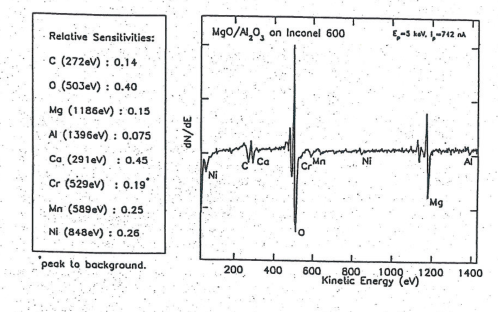
\includegraphics[scale=4]{figures/06_18.png}
	\caption{AES spectrum of interface between inconel 600 with a ceramic.}
	\label{fig:aesinconel}
	\end{center}
\end{figure}
\end{enumerate}
